% Generated by plsimcount.pffigure -- do not edit; regenerate instead.
% figure: A-measured-by-order -- Suzuki formulas of each order, r from: Measured $r$
% source: results/pf-thesis/results.json
% metric=cnot gatebase=cz merged
% seed=1 t=n template=simcount synth=pygridsynth
% git_commit=04cd66abb614bdc66fb48e891cef085a299e0ab1 git_dirty=False
% source_sha256=018e0b7603e6fc9f6ee358974f241415a3b93437700847b033937cc1d4250db8
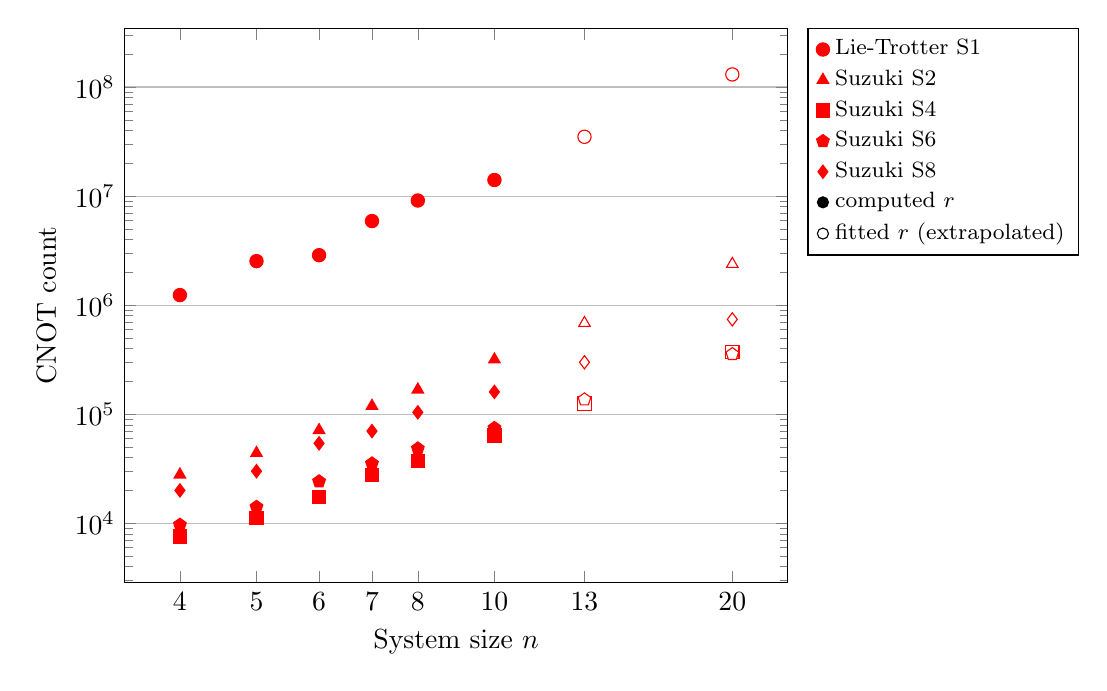
\begin{tikzpicture}
  \begin{loglogaxis}[
    width=10cm,
    xlabel={System size $n$},
    ylabel={CNOT count},
    xtick={4,5,6,7,8,10,13,20},
    xticklabels={4,5,6,7,8,10,13,20},
    ymajorgrids=true,
    legend pos=outer north east,
    legend cell align=left,
    legend style={font=\footnotesize},
  ]
    \addplot[only marks, red, mark=*, mark size=2.4pt, mark options={solid, fill=red}] coordinates {
      (4,1236768)
      (5,2534190)
      (6,2870640)
      (7,5902596)
      (8,9104160)
      (10,14037540)
    };
    \addlegendentry{Lie-Trotter S1}
    % r from power-law fit (extrapolation); one legend entry per series
    \addplot[only marks, red, mark=*, mark size=2.4pt, mark options={solid, fill=white}, forget plot] coordinates {
      (13,34960146)
      (20,130312080)
    };
    \addplot[only marks, red, mark=triangle*, mark size=2.4pt, mark options={solid, fill=red}] coordinates {
      (4,27960)
      (5,44050)
      (6,71340)
      (7,119070)
      (8,168160)
      (10,317400)
    };
    \addlegendentry{Suzuki S2}
    % r from power-law fit (extrapolation); one legend entry per series
    \addplot[only marks, red, mark=triangle*, mark size=2.4pt, mark options={solid, fill=white}, forget plot] coordinates {
      (13,685360)
      (20,2381200)
    };
    \addplot[only marks, red, mark=square*, mark size=2.4pt, mark options={solid, fill=red}] coordinates {
      (4,7560)
      (5,11130)
      (6,17388)
      (7,27636)
      (8,37296)
      (10,63840)
    };
    \addlegendentry{Suzuki S4}
    % r from power-law fit (extrapolation); one legend entry per series
    \addplot[only marks, red, mark=square*, mark size=2.4pt, mark options={solid, fill=white}, forget plot] coordinates {
      (13,125580)
      (20,371280)
    };
    \addplot[only marks, red, mark=pentagon*, mark size=2.4pt, mark options={solid, fill=red}] coordinates {
      (4,9696)
      (5,14140)
      (6,24240)
      (7,35350)
      (8,48480)
      (10,74740)
    };
    \addlegendentry{Suzuki S6}
    % r from power-law fit (extrapolation); one legend entry per series
    \addplot[only marks, red, mark=pentagon*, mark size=2.4pt, mark options={solid, fill=white}, forget plot] coordinates {
      (13,136552)
      (20,355520)
    };
    \addplot[only marks, red, mark=diamond*, mark size=2.4pt, mark options={solid, fill=red}] coordinates {
      (4,20040)
      (5,30060)
      (6,54108)
      (7,70140)
      (8,104208)
      (10,160320)
    };
    \addlegendentry{Suzuki S8}
    % r from power-law fit (extrapolation); one legend entry per series
    \addplot[only marks, red, mark=diamond*, mark size=2.4pt, mark options={solid, fill=white}, forget plot] coordinates {
      (13,299598)
      (20,741480)
    };
    \addlegendimage{only marks, black, mark=*, mark options={fill=black}}
    \addlegendentry{computed $r$}
    \addlegendimage{only marks, black, mark=*, mark options={fill=white}}
    \addlegendentry{fitted $r$ (extrapolated)}
  \end{loglogaxis}
\end{tikzpicture}
